\documentclass{article}
\usepackage[utf8]{inputenc}
\usepackage[russian]{babel}
\usepackage{listings}
\usepackage{graphicx}
% \usepackage{svg}

\title{Тема 21. Работа с массивами С++. Адресная арифметика.}
\author{Селиванова Вера}
\date{Декабрь 2016}

\begin{document}

\maketitle

\pagebreak



\section{Задача}

В матрице А(4,4), содержащей вещественные элементы, в каждом столбце поменять местами максимальный элемент с диагональным. Распечатать:

а) исходную и преобразованную матрицы;

б) адреса и значения тех элементов, которые оказались максимальными.

\pagebreak



\section{Программный код}

\lstinputlisting[language=C++]{sources/main.cpp}

\pagebreak



\section{Результат работы}

\lstinputlisting{result/output.txt}

\pagebreak



\section{Блок схема}

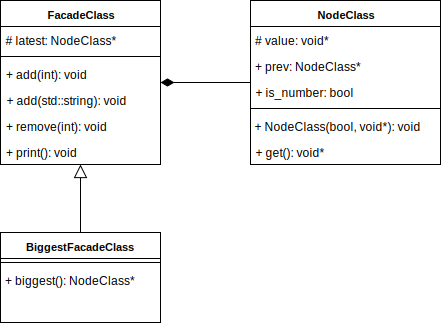
\includegraphics[scale=0.5]{result/scheme.png}

\end{document}

